\section{Eseguire A-CLus Base}

\subsection*{Operazioni preliminari}


\subsection*{Avvio dell'applicazione}

Per inizializzare correttamente la versione standard di A-CLus, attenersi alla seguente sequenza operativa:


\begin{enumerate}
    \item Accedere alla directory \texttt{A-CLus\_Base/Bat}
    \item Eseguire il file \texttt{Start\_Server.bat} facendo un doppio click su di esso, assicurandosi che venga mostrato il seguente messaggio a finestra
    
    \begin{figure}[h!]
        \centering
        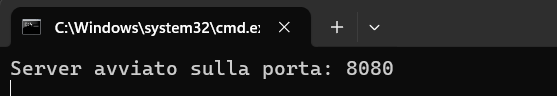
\includegraphics[width=0.5\textwidth]{images/server in esecuzione.png}
    \end{figure}

    \item Dopo aver verificato il corretto funzionamento del server, eseguire il file \texttt{Start\_Client.bat} facendo un doppio click su di esso; se non ci sono problemi con il server, apparirà la seguente schermata:
    
    \begin{figure}[h!]
        \centering
        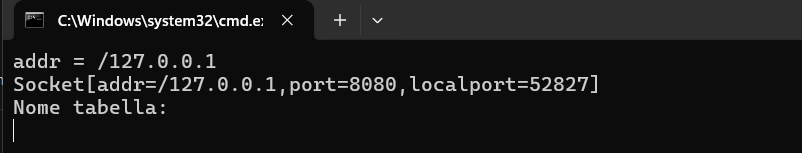
\includegraphics[width=0.5\textwidth]{images/client in esecuzione.png}
        
    \end{figure}
    
\end{enumerate}

\begin{tcolorbox}[colback=white, colframe=gray, title=Avvertenza]
    È necessario mantenere attivo il terminale del server per garantire la comunicazione tra le componenti client e server.
\end{tcolorbox}

\subsection*{Avvio dell'ambiente di sviluppo}

Per aprire correttamente il codice sorgente di A-CLus, è necessario seguire le seguenti operazioni nell'ordine in cui sono presentate:

\begin{enumerate}
    \item Aprire la cartella del progetto \texttt{A-Clus\_base}
    \item Incorporare nelle librerie del progetto \texttt{Server} il file \texttt{mySQL\_connector.jar} presente nella cartella \texttt{A-CLus/Risorse}. Nel caso si stia eseguendo il progetto in Visual Studio Code, è possibile eseguire i seguenti passaggi:
    \begin{enumerate}
        \item Aprire il progetto \texttt{A-Clus\_Base}
        \item Recarsi nella sezione \texttt{Referenced Libraries}, in asso a sinistra
        \item Posizionare il cursore sulla cartella e selezionare \texttt{Add JAR/Folder Classpath}, che apparirà sulla destra
        \begin{figure}[h!]
            \centering
            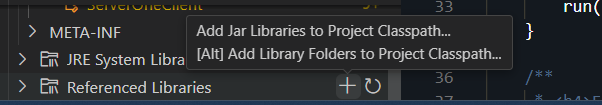
\includegraphics[width=0.5\textwidth]{images/refenereziare il jdbc.png}
        \end{figure}
    \end{enumerate}
    \item Avviare \texttt{MultiServer.java}
    \item Controllare che il server sia in esecuzione correttamente
    \item Aprire il progetto \texttt{MainTest.java} presente nella cartella \texttt{A-CLus\_Base/Client}
\end{enumerate}

\subsection{Interfaccia iniziale}

L'interfaccia iniziale di A-CLus è composta da tre sezioni principali:

\begin{figure}[h!]
    \centering
    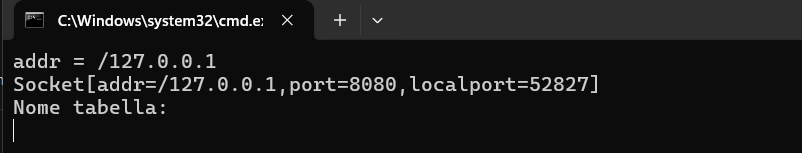
\includegraphics[width=\textwidth]{images/client in esecuzione.png}
    \caption{Interfaccia iniziale di A-CLus}
\end{figure}



